\chapter{Introduction}\label{sec:intro}
In this chapter, the problem addressed by this Master Thesis is introduced. First, the bridge type and its characteristics are described in \cref{sec:int_back}, complemented by a brief historical integration. In \cref{sec:int_prob}, the problem is stated and defined. Ultimately, an outline of the Thesis is given \cref{sec:int_out}.

\section{Background}\label{sec:int_back}
Network tied-arch bridges serve the same function as simply supported beams by spanning a single field supported on vertical bearings at its ends, of which one is horizontally restricted. Compared to a simple beam, which carries the loads on internal bending moments, the tied-arch bridge forms a truss structure featuring a tension and a compression chord to carry the global bending moment. The tie girder forms the tension chord tying the arch ends and supporting its horizontal forces. The deck may be integrated into the tie girder (composite deck system) or be supported vertically on deck floor beams (floating deck system). The arches are arranged in planes which can either be vertical or inclined. Each plane usually features two hanger sets, which connect the tie and the arch and cross each other multiple times. The structural components for a floating deck system are illustrated in \cref{fig:components_illustration}.
\begin{figure}[H]
    \centering
    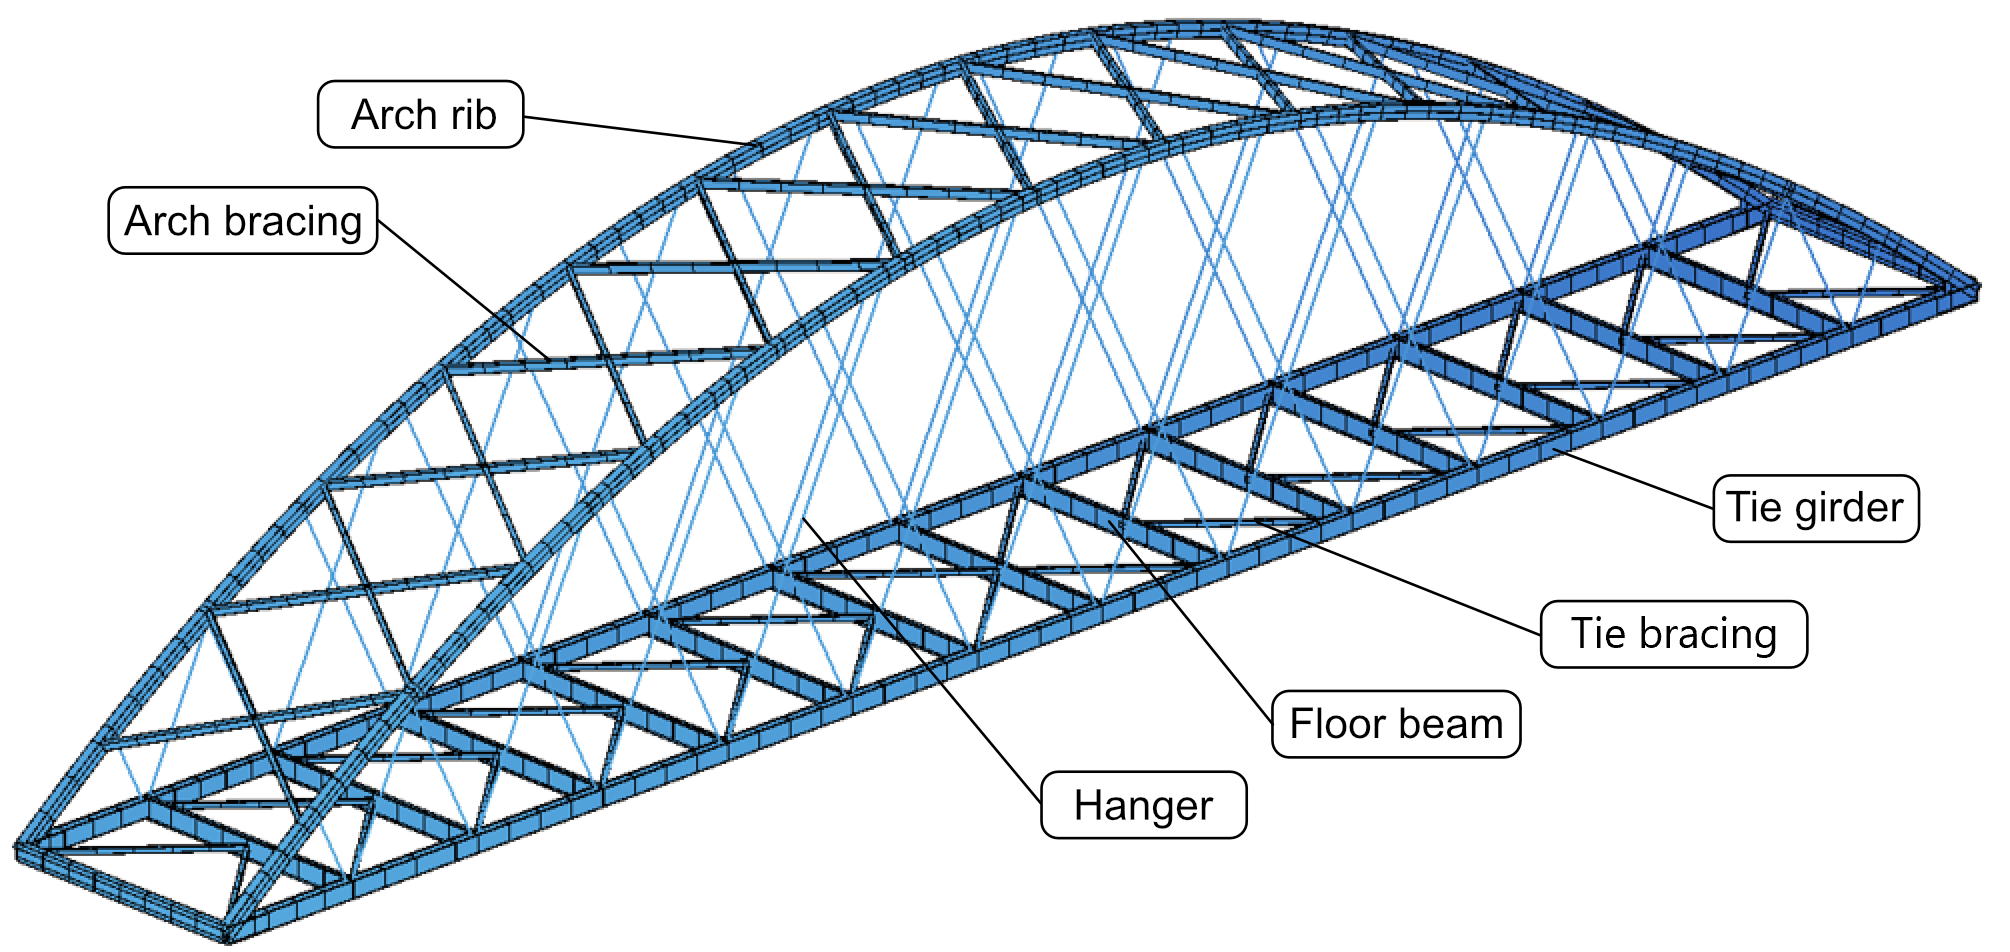
\includegraphics[width=0.65\textwidth]{overleaf/Pictures/illustration_components.PNG}
    \caption{Structural components of a network tied-arch bridge}
    \label{fig:components_illustration}
\end{figure}

The network tied-arch bridge is considered an enhanced construction scheme offering aesthetic appeal and benefits in terms of structural efficiency \cite{Hu}. Steel bridges of this type require significantly less material and allow for more slender cross-sections than other more popular bridge-types \cite{Herzog}. However, network tied-arch bridges can be considered a complex structural system and the associated challenges are broad and demanding. 
The hanger arrangement and its initial configuration influence the behaviour under asymmetric live loading, fatigue and cable loss. 
Many of these challenges have not been satisfactorily addressed \cite{Bruno_2}. Other design variables such as the arch shape and its rise as well as its bracing and inclination have barely been studied. Nevertheless, a strong surge in the popularity of this bridge-type is observed in the last two decades, as shown in \cref{fig:yearly_bridges}.

\begin{figure}[H]
    \centering
    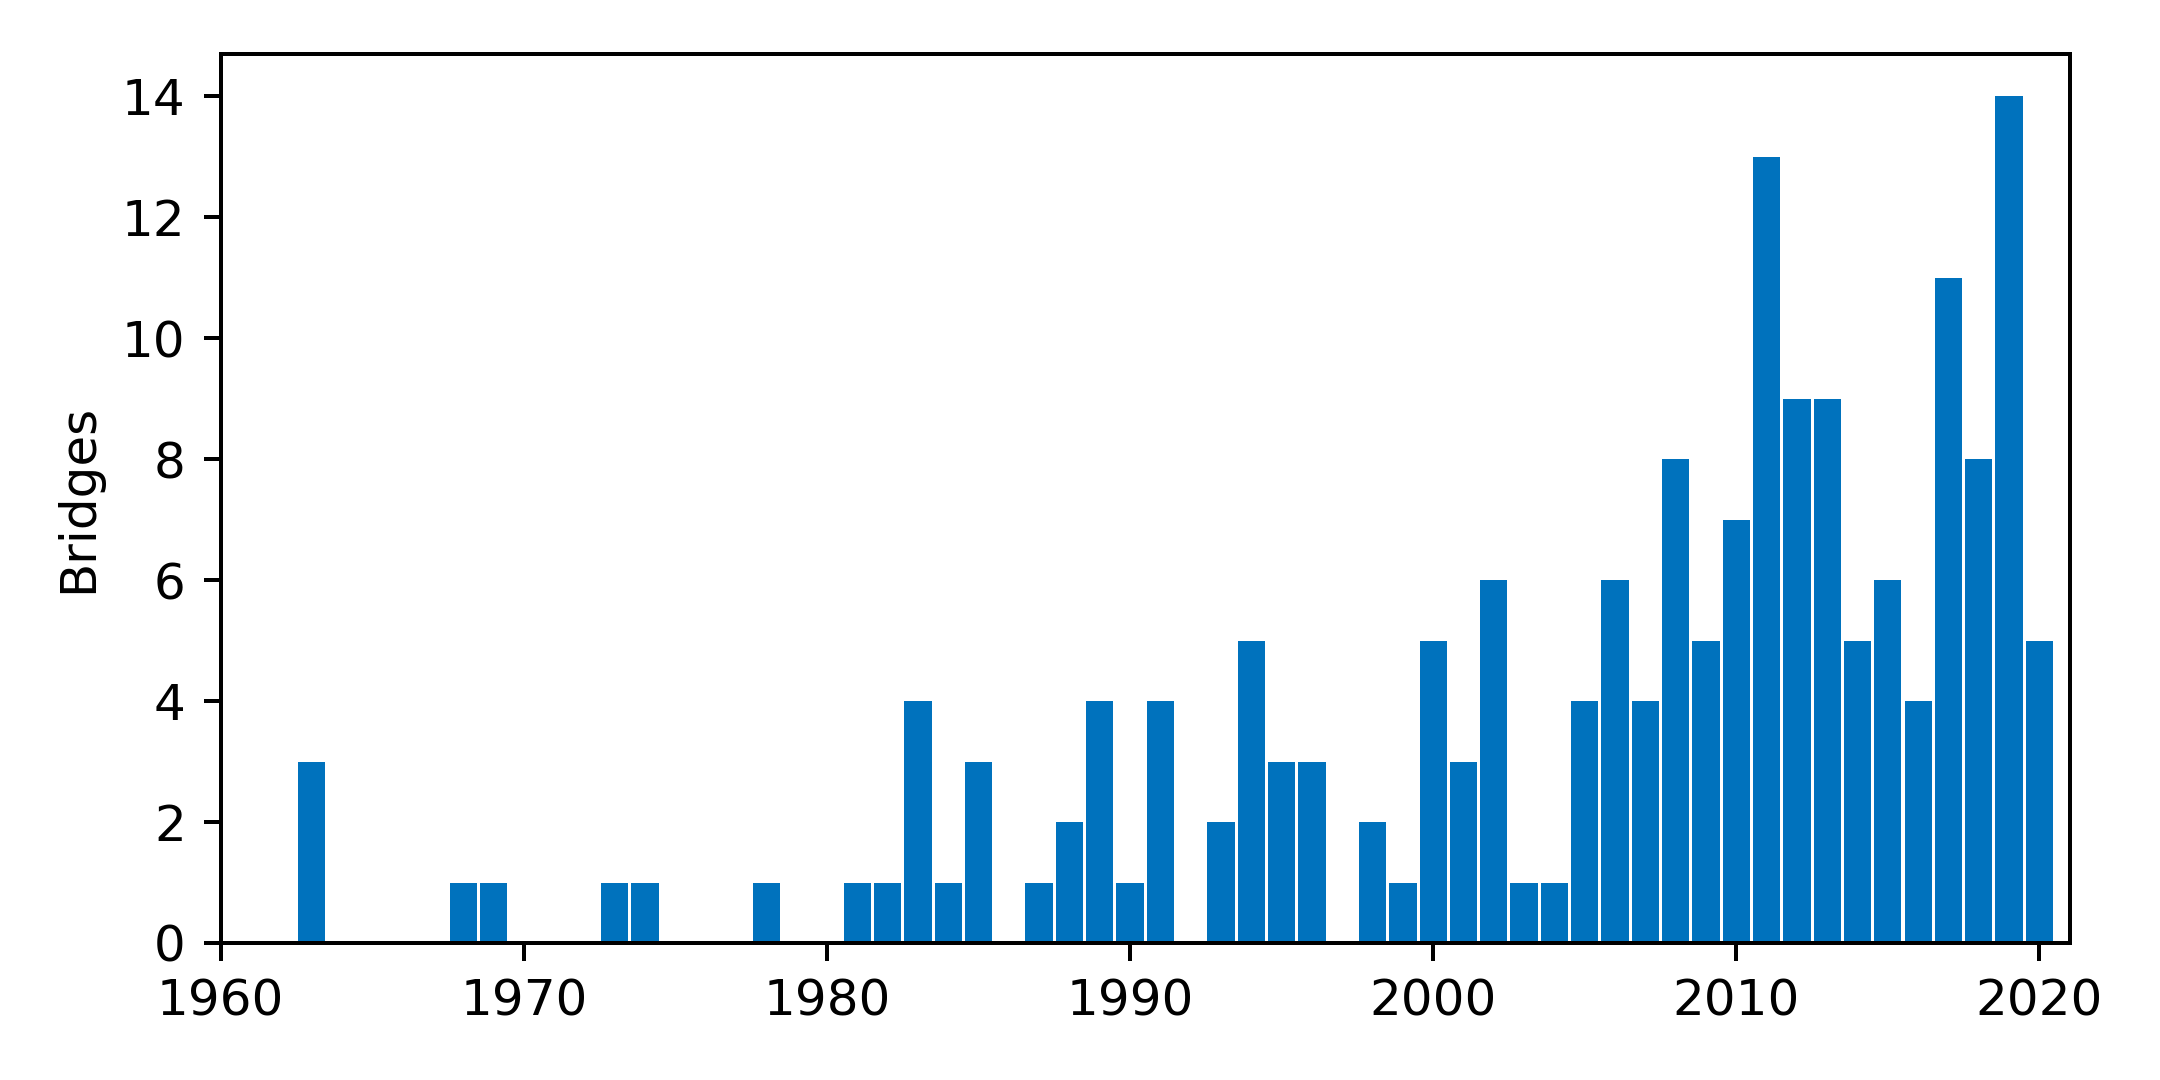
\includegraphics[trim={0 2.2cm 0 1.8cm},clip, width=0.60\textwidth]{overleaf/Pictures/myplot.png}
    \caption{Number of network tied-arch bridges built per year \cite{Cavegn}}
    \label{fig:yearly_bridges}
\end{figure}

The origin of this bridge type can be traced back into the 19th century when multiple engineers started designing tied-arch bridges featuring a tension chord in the tie. Among these engineers are Joseph Langer and Hermann Lohse who arranged the hangers vertically as shown in \cref{fig:langerscherbalken}. In the 1920s, the Danish engineer Octavius F. Nielsen recognised the advantages of inclined hangers, which significantly reduce the longitudinal bending moments and thereby allow for longer spans. Despite showing intersecting hangers in his patent document, he only designed hanger arrangements without intersections \cite{Tveit_Bits}. The structural analysis of a bridge with intersecting hangers was too challenging at the time. Besides that, he struggled with hanger loss due to unloading. One of his bridges is presented in \cref{fig:nielsenbridge}.

\begin{figure}[H]
\centering
\begin{minipage}{.5\textwidth}
  \centering
  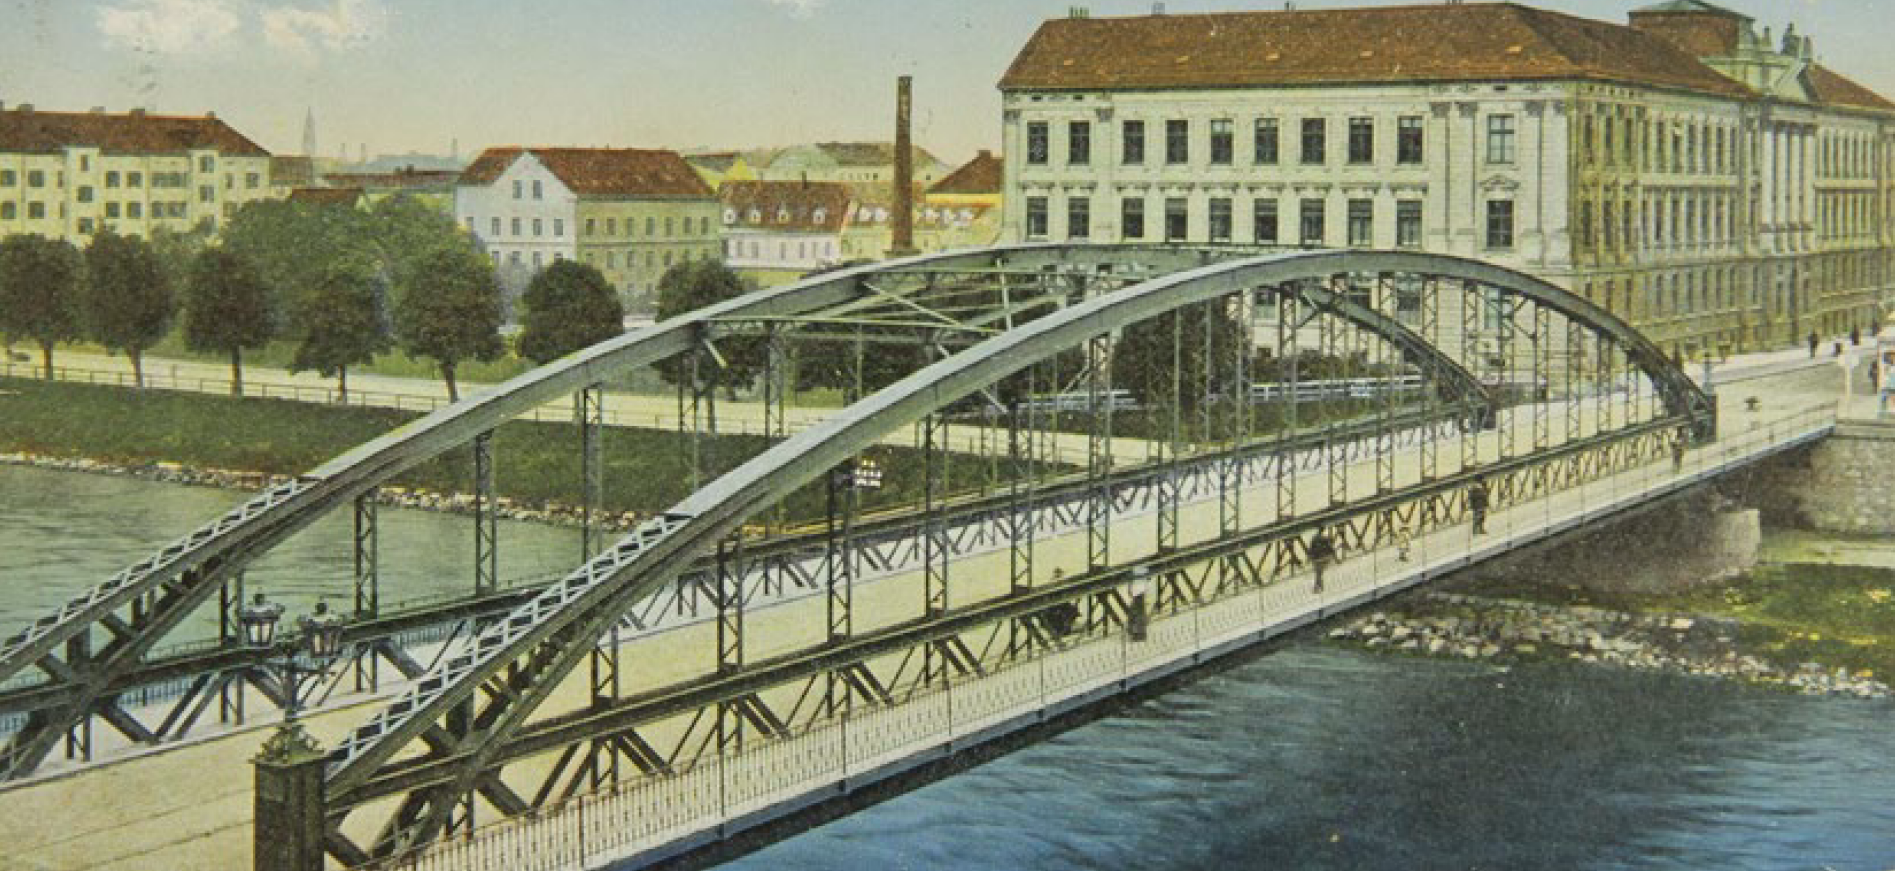
\includegraphics[width=.9\textwidth]{overleaf/Pictures/langerscher balken.PNG}
  \captionof{figure}{Old Ferdinandbridge \cite{Langer}}
  \label{fig:langerscherbalken}
\end{minipage}%
\begin{minipage}{.5\textwidth}
  \centering
  \vspace*{0.6cm}
  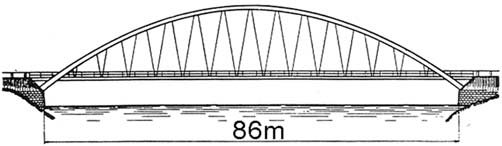
\includegraphics[width=.9\textwidth]{overleaf/Pictures/Nielsen bridge.png}
  \vspace*{0.6cm}
  \captionof{figure}{Nielsen bridge \cite{Nielsen}}
  \label{fig:nielsenbridge}
\end{minipage}
\end{figure}

As the live loading increased in the following years, Nielsen bridges became less suitable. Only by intersecting the hangers, flat hanger inclinations could be obtained, which solves the problem of hanger unloading. The network tied-arch bridge featuring hangers with multiple intersections was introduced by Per Tveit in 1955. The first bridges of this type were built in 1963. One of them, the Fehmarn Sound Bridge, which already spanned \SI{248}{m}, is shown in \cref{fig:Fehmarnsundbrcke}.

\begin{figure}[H]
    \centering
    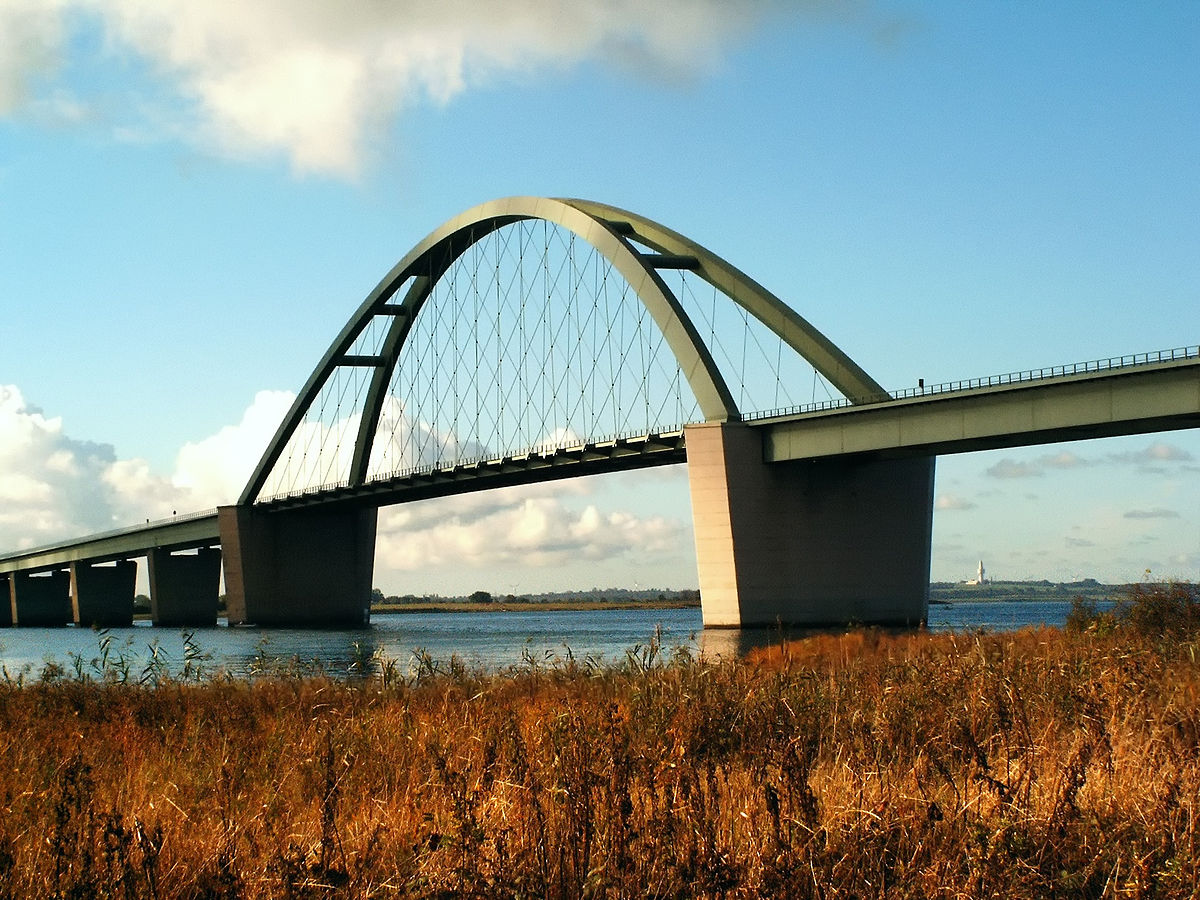
\includegraphics[trim={0 1.5cm 0 0.7cm},clip, width=0.55\textwidth]{overleaf/Pictures/Fehmarnsund.jpg}
    \caption{Fehmarn Sound Bridge \cite{Fehmarnsund}}
    \label{fig:Fehmarnsundbrcke}
\end{figure}

In the following decades, Per Tveit focused his research on this bridge type, emphasising the importance of the hanger inclination. Despite his efforts, no more bridges of this type were built in Europe until the end of the millennium. However, the idea was exported to Japan, where it became a standard alternative to classic tied-arch bridges and over 50 bridges of this type were built for medium spans. In the last two decades, researchers and engineers developed more interest in this bridge type, which has now been built more than 200 times around the world. The Blennerhassett Island Bridge, shown in \cref{fig:Blennerhassett}, is a particularly large example, which serves as a reference for the investigations in this Thesis.

\begin{figure}[H]
    \centering
    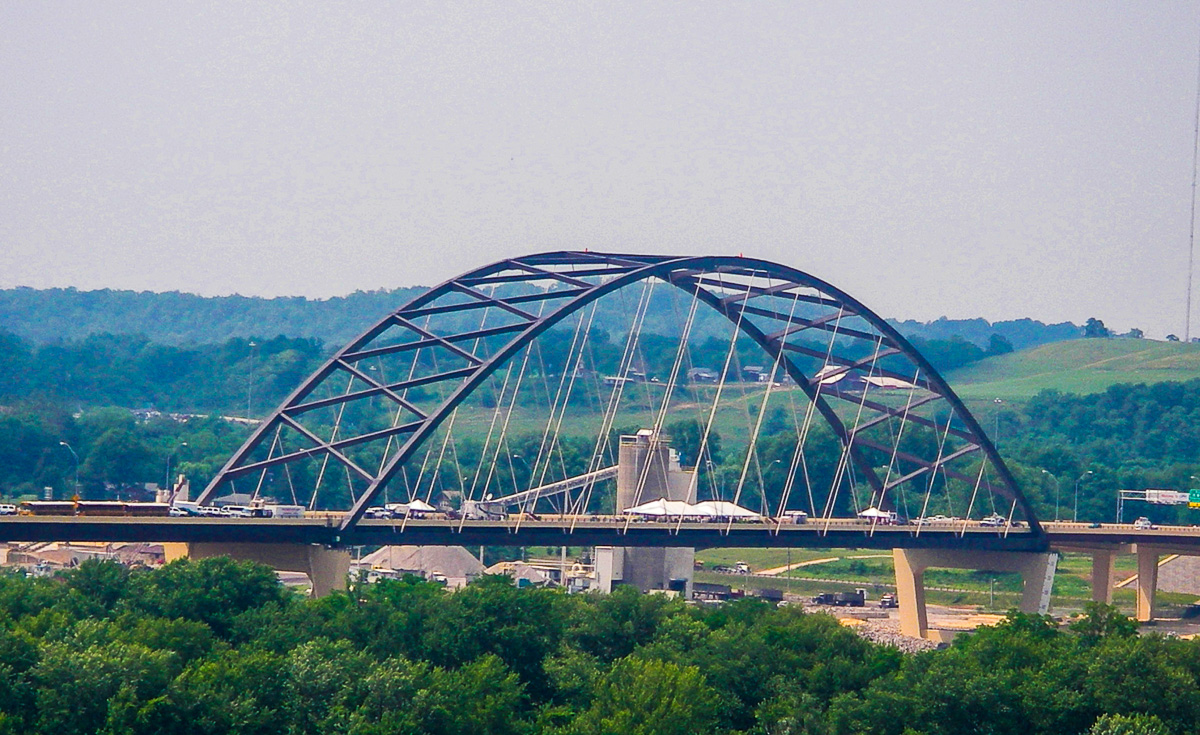
\includegraphics[width=0.6\textwidth]{overleaf/Pictures/Blennerhassett.jpg}
    \caption{Blennerhassett Island Bridge \cite{Blennerhassett}}
    \label{fig:Blennerhassett}
\end{figure}

\section{Problem statement} \label{sec:int_prob}
Network tied-arch brides are complex structural systems with much freedom in their articulation.
They are characterised by the arch shape, its inclination and bracing, the hanger arrangement, the hanger density and the deck system. Many of these design variables can be freely chosen, opening up a vast space of possible designs. 
For its very efficient use of the utilised materials, an increase in its usage is preferable for the future. Therefore, design guidelines and investigations of the critical aspects are necessary to facilitate efficient initial designs.
This Master Thesis is part of a series of projects on the optimisation of network tied-arch bridges at the institute of structural engineering at ETH Zurich. As the full optimisation of this bridge type covers too many aspects for a single Thesis, different focal points are investigated independently. A previous Master Thesis carried out by Riccardo Cavegn investigated the arch geometry, the self-equilibrium stress state and the hanger arrangements \cite{Cavegn}. 
The present Thesis relies on this previous work using similar methods and facing many identical challenges.
In this Thesis, the emphasis lies in the investigation of the hanger density and the hanger inclination. It is investigated whether an increased number of hangers can improve the bridge's structural behaviour, particularly in combination with the radial hanger arrangement. Therefore, the derivation of the self-equilibrium stress state is of critical relevance. Further, the choice of the arch shape is subject to the investigation as the arch rib's demand depends on the hanger arrangement. Ultimately, also the hanger inclination is investigated to put this critical parameter into the perspective of an integral design verification.
The Blennerhassett Island Bridge serves as a reference for the investigations. It is an impressive structure designed mainly for structural efficiency, which frames the objective in this Thesis.  

\section{Outline} \label{sec:int_out}
In \cref{sec:review}, the previous literature in the field of network tied-arch bridges is summarised. However, many relevant aspects have barely been considered in the past. Therefore, a wide range of topics is covered to give a general overview of the field and the commonly used methods. The reference bridge, the design verifications and the optimisation methods used in this investigation are introduced in \cref{sec:methods}. It first introduces the Blennerhassett Island Bridge, the structural model and its underlying assumptions. Further, the load cases and limit states considered for the design verifications are presented. Also, new methodologies for the derivation of an efficient arch shape and self-equilibrium stress state are introduced. Ultimately, the estimation of the costs associated with a particular design is given. The results of the different investigated aspects are given in \cref{sec:results}. First, the base case of the Blennerhassett Island Bridge's final design is derived, followed by the investigation of the arch shape using the new methodology. Further, the hanger and the floor beam density is investigated. Finally, the influence of the hanger inclination on the structural behaviour is shown, and the chapter is briefly summarised. The results are concluded in \cref{sec:conclusion} by giving practical design guidelines. Also, an outlook for further research is given in \cref{sec:outlook}. For unknown terms and citations, the glossary and the references are given before the Appendix.

\section{Terminology}
\begin{description}
    \item[Arch shape]
    \item[Constant change arrangement] Test
    \item[Design condition]
    \item[Evolutionary algorithm]
    \item[Hanger arrangements]
    \item[Hanger inclination]
    \item[Hanger set]
    \item[Knuckle]
    \item[Linear programming problem]
    \item[Objective function] Most optimisation methods require the definition of a single function to rank the optimality of a specific design. The optimisation method tries to find design which yields the minimum value for this function.
    \item[Parallel arrangement]
    \item[Knuckle]
    \item[Radial arrangement]
    \item[Self-equilibrium stress state]
    \item[Zero-displacement method]
\end{description}
